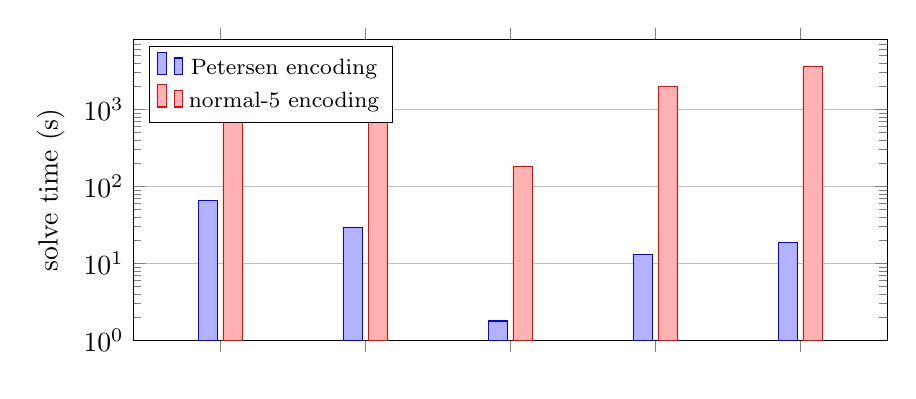
\begin{tikzpicture}
\begin{axis}[ybar, bar width=7pt, width=0.92\textwidth, height=5.4cm, ymode=log, log origin=infty,
 symbolic x coords={G112,H112,G52,G52p,G68}, xtick=data, xticklabels={$\Gmain$,$\Gsym$,$\Gfty$,$\Gftyb$,$\Gsix$}, x tick label style={font=\footnotesize}, ylabel={solve time (s)}, ymin=1, ymax=8000,
 legend style={at={(0.02,0.98)},anchor=north west,font=\footnotesize}, enlarge x limits=0.15, ymajorgrids]
\addplot coordinates {(G112,65.643) (H112,29.476) (G52,1.789) (G52p,13.116) (G68,18.879)};
\addplot coordinates {(G112,1216.819) (H112,977.188) (G52,178.798) (G52p,1977.826) (G68,3588.662)};
\legend{Petersen encoding, normal-5 encoding}
\end{axis}
\end{tikzpicture}
